\section{Zielsetzung}
Im Versuch soll überprüft werden, ob die Molwärmen verschiedener Stoffe mit Hilfe
des Dulong-Petitschen Gesetzes ermittelt werden können, oder ob es quantenmechanischer
Berechnungen bedarf, um diese genauer zu bestimmen.

\section{Theorie}
Das Dulong-Petitsche Gesetz besagt, dass die Molwärme in Festkörpern, stoffunabhängig,
stets 3R beträgt, wobei $R \approx 8,314 \frac{J}{mol K} $ die ideale Gaskonstante ist.
Dies lässt sich mit Hilfe einiger Gesetze aus der klassischen Mechanik, wie
Energieerhaltung oder der Annahme, dass Atome in festen Körpern annähernd wie
harmonische Oszillatoren schwingen, herleiten.
Bei hohen Temperaturen kann beobachtet werden, dass das Dulong-Petit'sche Gesetz für alle festen
chemischen Elemente seine Gültigkeit besitzt. Dies ist meist schon bei Zimmertemperatur der Fall.
Lediglich leichte Elemente, wie Bor oder Beryllium, müssen auf bis zu $\SI{1000}{\degree}$ erhitzt
werden, um das Gesetz zu erfüllen.
Die Energie der Atome beträgt dann:
\begin{align*}
  E = 3 \symup{R T} .
\end{align*}
\FloatBarrier
Werden jedoch sehr tiefe Temperaturen betrachtet, so ist zu erkennen, dass die Molwärmen aller
chemischen Elemente beliebig klein werden. Dieses Phänomen ist mit der klassischen
Physik nicht zu erklären, weshalb es der Quantenmachanik bedarf.
Hierbei liegt die Annahme zu Grunde, dass ein mit der Frequenz $\omega$ oszillierendes Atom nur diskrete
Energiewerte annehmen kann:
\begin{align*}
  \Delta E = n \cdot \hbar \cdot \omega
\end{align*}
Für die gemittelte Energie ergibt sich somit ein nicht mehr linearer Zusammenhang
zwischen Energie und Temperatur:
\begin{align*}
  E = \frac{3 N_A \hbar \omega}{\exp{\frac{\hbar \omega}{k \symup{T}}}-1} .
\end{align*}
Hier ist auch zu erkennen, dass für hohe Temperaturen $k\symup{T} \gg \hbar \omega$
die Energie wiederum 3RT beträgt.


\noindent
Mit der Mol- oder Atomwärme ist die Menge Wärme dQ gemeint, die erforderlich ist, um ein
Mol eines chemischen Elements um dT zu erwärmen. Die Molwärme eines Elements bei
konstantem Volumen (V) oder bei konstantem Druck (P) ist:
\begin{align*}
  C_\symup{V} = \left(\frac{\symup{dQ}}{\symup{dT}}\right)_\symup{V}  &&& C_\symup{P} = \left(\frac{\symup{dQ}}{\symup{dT}}\right)_\symup{P}
\end{align*}
und beschreibt die Fähigkeit eines Stoffes, Wärme zu speichern.

Mit Hilfe folgender Gleichung kann die Molwärme eines Stoffes, $C_\symup{V}$, einfach
berechnet werden, was experimentell zu bestimmen deutlich komplizierter wäre, da
es hoher externe Drücke bedarf, um Stoffe auf einem konstanten Volumen zu halten:
\begin{equation}\label{eq1}
  C_\symup{V} = c_\symup{K} \cdot M - 9 \alpha^2 \kappa \frac{M}{\rho} \symup{T}
\end{equation}
Hierbei steht $\alpha$ für den linearen Ausdehnungskoeffizienten, $\kappa$ für das Kompressionsmodul, $\rho$ für die Dichte
und $M$ für die molare Masse, welche materialspezifische Konstanten sind.
Die spezifische Wärmekapazität $c_\symup{K}$ ist ein Proportionalitätsfaktor,
der bestimmt, wieviel Wärme vom Körper bei einer Änderung der Temperatur abgegeben wird:
\begin{align*}
  \Delta Q = M c_\symup{K} \Delta T
\end{align*}

Mit folgender Formel lässt sich nun die spezifische Wärmekapazität eines Probenmaterials bestimmen:
\begin{align}
  \label{eq3}
  \symup{c}_\symup{k} = \frac{(\symup{c}_\symup{w}\symup{m}_\symup{w} + \symup{c}_\symup{g}\symup{m}_\symup{g})(\symup{T}_\symup{m}\symup{T}_\symup{w})}{\symup{m}_\symup{k}(\symup{T}_\symup{k} - \symup{T}_\symup{m})}
\end{align}
Alle in der Gleichung angegebenen Werte lassen sich ermitteln.
Lediglich für $\symup{c}_\symup{g}\symup{m}_\symup{g}$, der spezifischen Wärmekapazität des Kalorimeters, bedarf es
einer weiteren Berechnung. Es werden zwei Wassermengen $\symup{m}_x$ und $\symup{m}_y$ mit
den Temperaturen $\symup{T}_x$ und $\symup{T}_y$ miteinander vermischt und
die sich einstellende Mischtemperatur $\symup{T}_m$ gemessen.
\begin{equation}\label{eq2}
  \symup{c}_\symup{g}\symup{m}_\symup{g} = \frac{\symup{c}_\symup{w}\symup{m}_y (\symup{T}_y - \symup{T}_m) - \symup{c}_\symup{w}\symup{m}_x (\symup{T}_m - \symup{T}_x)}{(\symup{T}_m - \symup{T}_x)}
\end{equation}
\newpage
\section{Durchführung}
Der Versuchsaufbau ist in Abb.\ref{abb1} zu sehen. Zur Durchführung wird ein Kalorimeter,
eine Heizplatte, verschiedene Gefäße, in denen Wasser erhitzt oder umgefüllt werden kann, eine
Schnellwaage und ein Thermometer benötigt.
\begin{figure}
  \centering
  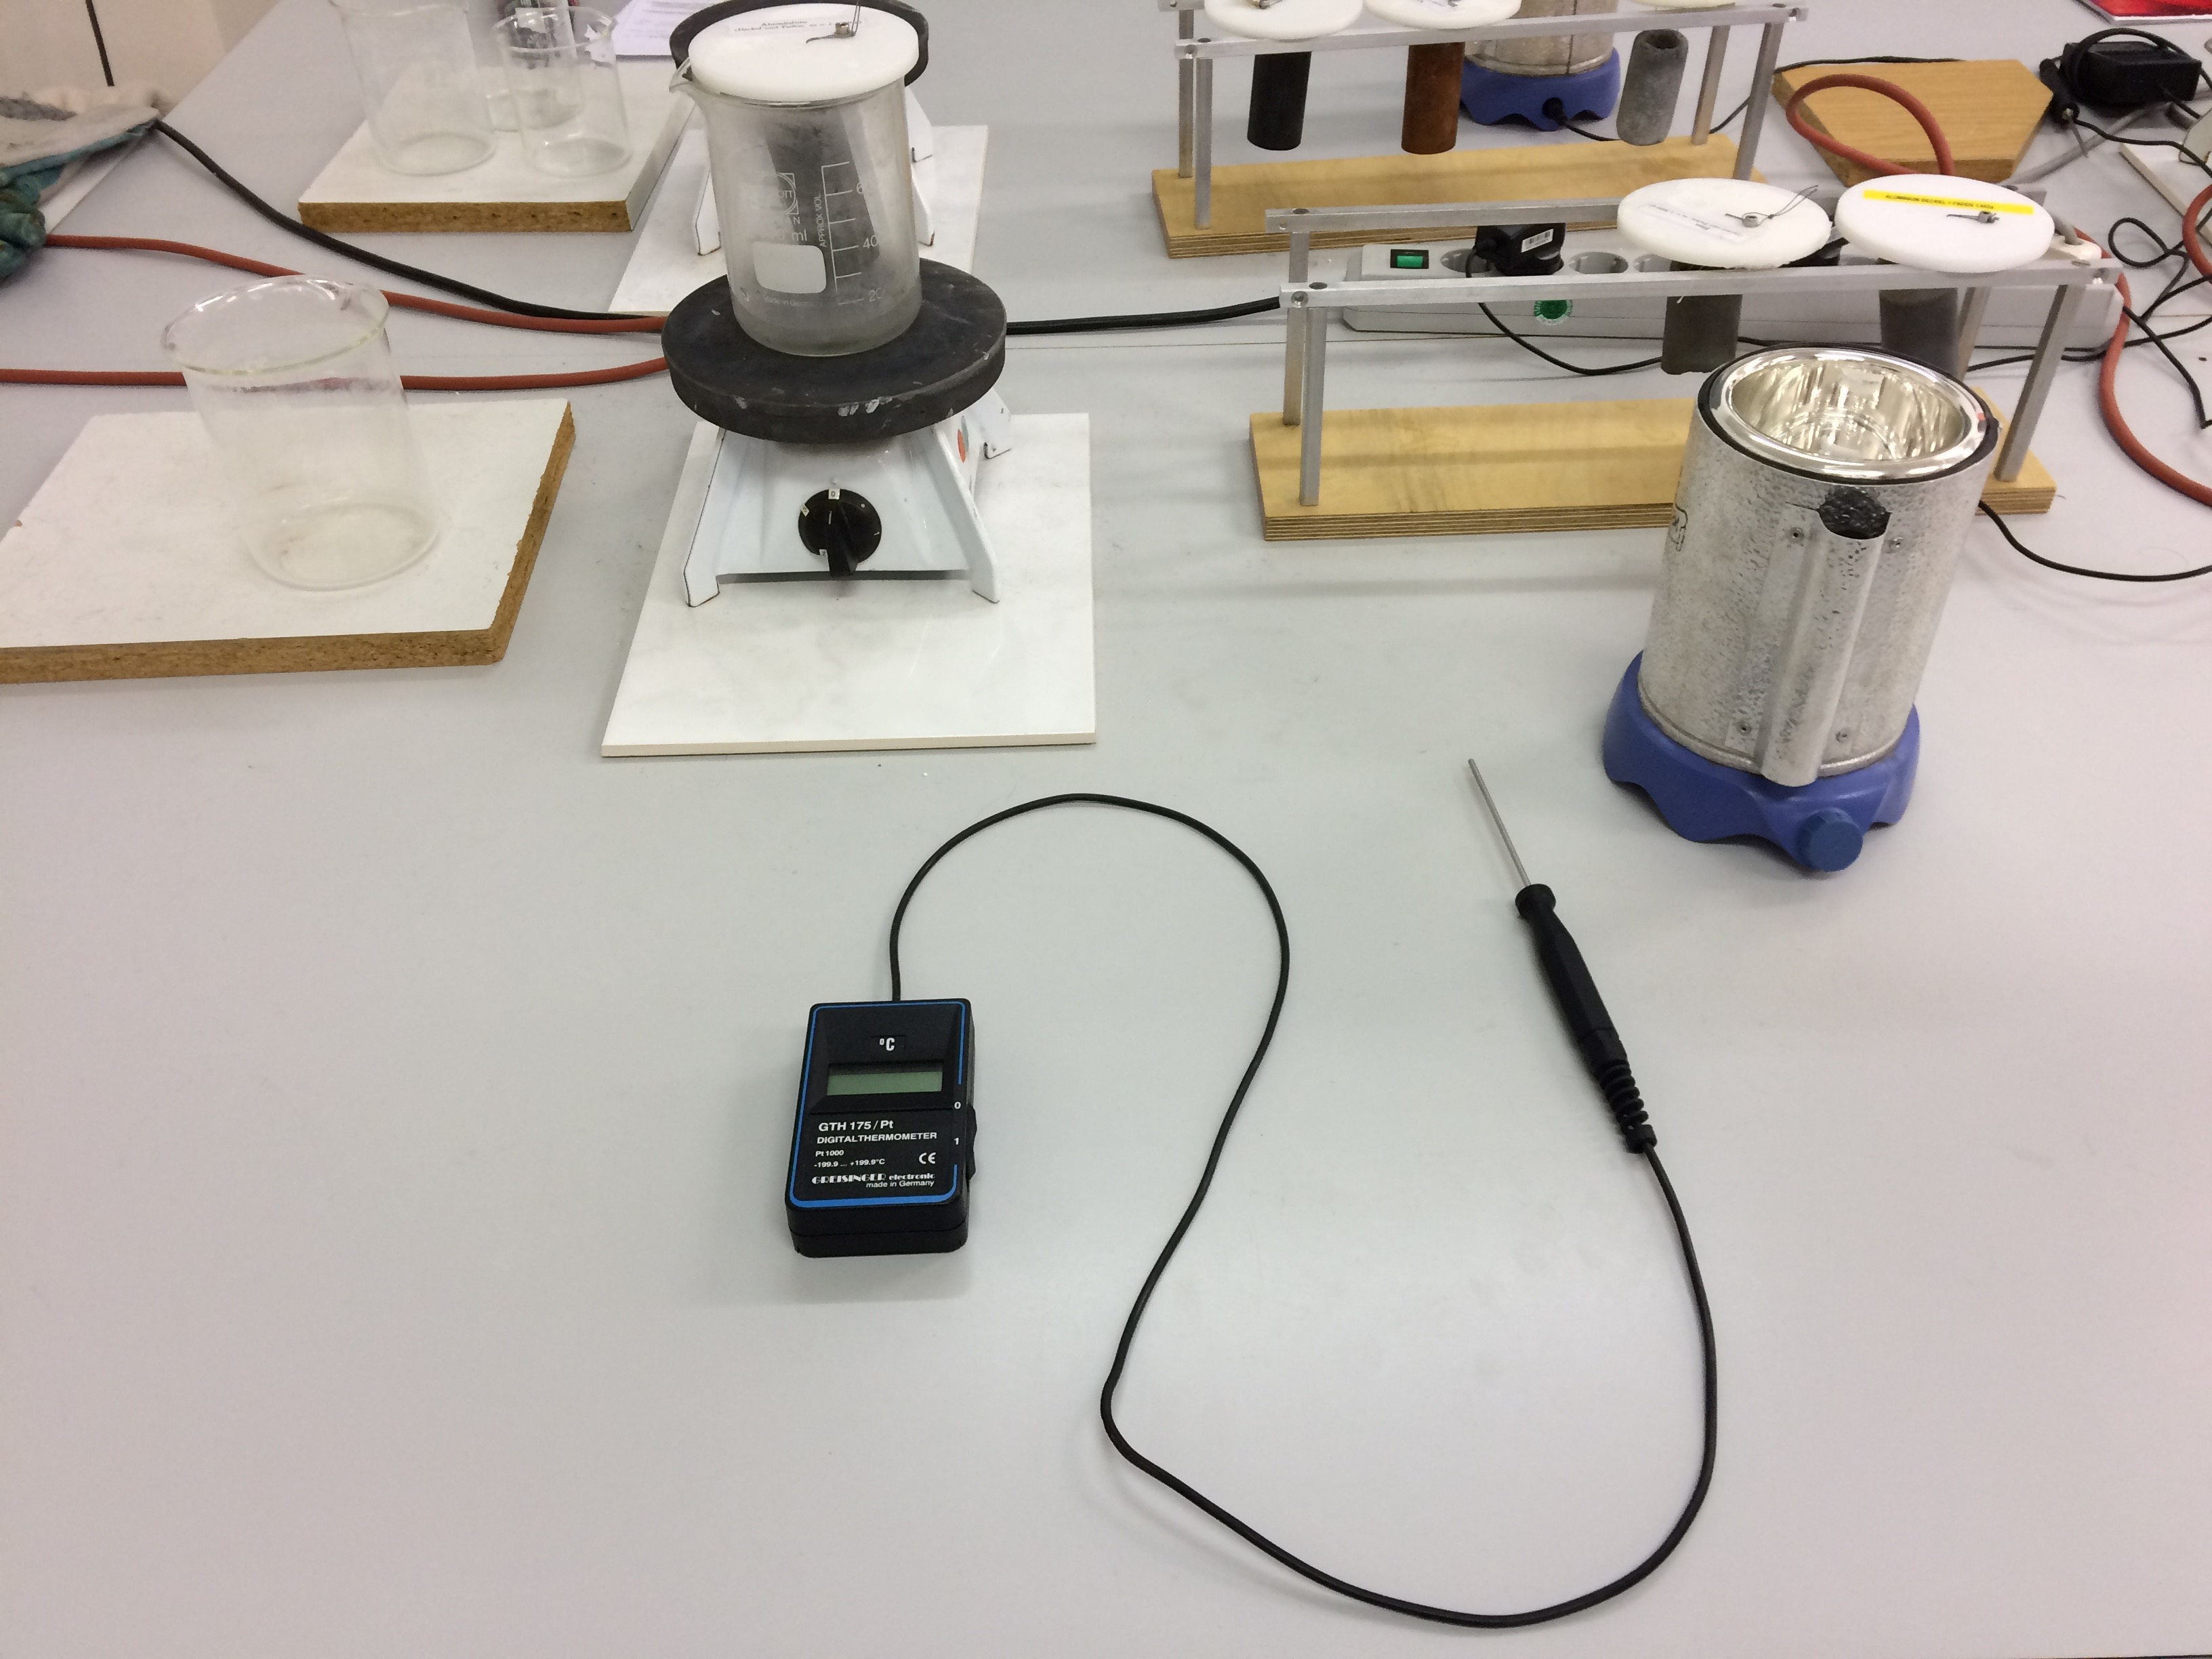
\includegraphics[scale=0.07]{Aufbau.jpg}
  \caption{Versuchsaufbau}
  \label{abb1}
\end{figure}
\FloatBarrier
Im ersten Teil des Versuchs wird die spezifische Wärmekapazität des Kalorimeters ermittelt.
Hierfür wird eine Hälfte einer Wassermenge $\symup{m}_x$ , die die Temperatur $\symup{T}_x$
hat, in ein Kalorimeter gegeben. Die andere Hälfte $\symup{m}_y$ mit der Temperatur $\symup{T}_y$
wird auf einer Heizplatte auf annähernd $\SI{100}{\degree}$ erhitzt. Sobald eine Temperatur von
$\SI{100}{\degree}$ erreicht ist, wird die Menge $\symup{m}_y$ zu Menge $\symup{m}_x$ in das
Kalorimeter gegossen. Das Wasser wird ausreichend verrührt und anschließend die Mischtemperatur
gemessen. Die beiden Wassermengen werden mittels einer Schnellwaage bestimmt und sollten ungefähr
gleich groß sein.
Mit Hilfe der spezifischen Wärmekapazität von Wasser $\symup{c}_\symup{w} = \SI{4,18}{\J \per \gram \per \K}$
und Gleichung \eqref{eq2} kann nun die spezifische Wärmekapazität des Kalorimeters berechnet werden.


\noindent
Im weiteren Verlauf des Versuchs werden nun Molwärmen verschiedener Stoffe bestimmt.
Dazu muss zunächst die spezifische Wärmekapazität der verschiedener Proben, hier: Graphit, Zinn und Aluminium bestimmt
werden, aus dieser und mit Hilfe von Gleichung \eqref{eq1} kann dann die Molwärme der Proben
berechnet werden. Die errechneten Ergebnisse können anschließend mit der Aussage des
Dulong-Petitschen Gesetzes verglichen werden.

\noindent Es wird zunächst die Masse $\symup{m}_\symup{k}$ der einzelnen Proben mittels Schnellwaage bestimmt.
Hierbei ist zu beachten, dass die Proben an einem Deckel befestigt sind,
sodass sie zum Erhitzen in ein Wasserbad eingetaucht werden können. Das Gewicht
des Deckels ist angegeben und muss nach dem Wiegen von der Gesamtmasse abgezogen werden.
Anschließend wird eine Wassermenge $\symup{m}_\symup{w}$ ebenfalls mit der Schnellwaage
gewogen und in ein Kalorimeter gegeben. Auch hier wird zuerst die Masse des Gefäßes
bestimmt, um diese dann von der Gesamtmasse abzuziehen. Folgend wird nach einer kurzen
Wartezeit, in der sich die Temperatur der Kalorimeterwand und die des eingegossenen Wassers
angeglichen haben, die Temperatur des Wassers im Kalorimeter gemessen.
Das Wasserbad, in dem sich die Probe befindet, wird anschließend auf der Heitzplatte
auf $\SI{100}{\degree}$ erhitzt. Die Probe kann dann aus dem Wasserbad genommen werden, um
dessen Temperatur $\symup{T}_\symup{k}$ zu bestimmen. Ist dies geschehen, wird die erhitzte
Probe in das Wasser im Kalorimeter eingetaucht. Es wird nun alternierend die Temperatur
des Wassers und der sich darin befindlichen Probe gemessen. Haben die Probe und das
Wasser die gleiche Temperatur, so wird diese Temperatur $\symup{T}_\symup{m}$ notiert.
Dieses Vorgehen wird nun drei mal jeweils für Graphit und Zinn wiederholt, um im Anschluss
eine Fehlerrechnung durchführen zu können.
Abschließend wird der Messvorgang einmal für Aluminium durchgeführt.


\section{Auswertung}
Die folgenden Rechnungen werden alle mit Python und die Tabellen mit Latex durchgeführt.
\subsection{Bestimmung der Wärmekapazität des Kaloriemeters}

Um später die spezifischen Wärmekapazität verschiedener Stoffe bestimmen zu können, ist es notwendig die
spezifische Wärmekapazität des Kalorimeters zu kennen.

Hierzu werden die gemessenen Werte aus Tabelle \ref{tab1} in die Gleichung \eqref{eq2} eingesetzt, mit
$c_w = \SI{4.18}{\joule\per\gram\per\kelvin}$ \cite{Quelle}.

\begin{table}
  \centering
  \caption{Messwerte zu Bestimmung der Wärmekapazität des Kalorimeters.}
  \label{tab1}
  \begin{tabular}{c c c c}
    \toprule
    $m_x$ / $\si{\gram}$ & $T_x$ / $\si{\celsius}$ &  $m_y$ / $\si{\gram}$ & $T_y$ / $\si{\celsius}$ \\
    \midrule
    287.00 & 22.5 & 274.55 & 98.9 \\
    \bottomrule
  \end{tabular}
\end{table}

Einsetzen liefert den folgenden Wert für $c_g m_g$ :

\begin{align*}
  c_g m_g = \SI{74.76}{\joule\per\kelvin}
\end{align*}

\subsection{Bestimmung der Molwärme verschiedener Stoffe}
Um die Molwärme berechnen zu können, wird zunächst zu jedem Stoff die spezifische Wärmekapazität berechnet
und daraus folgend die Molwärme.

\begin{figure}[h]
  \centering
  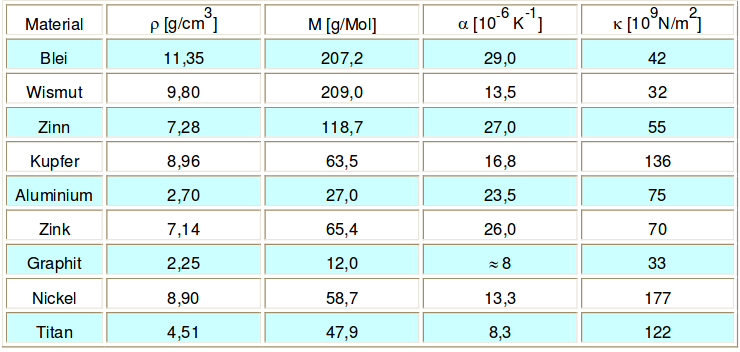
\includegraphics[scale = 0.5]{Tabelle.png}
  \caption{Physikalische Eigenschaften der verwendeten Probematerialien. \cite{Quelle}}
  \label{Abb2}
\end{figure}

\newpage
\subsubsection{Graphit}
Bei der Messung mit Graphit ergeben sich die Werte, die in Tabelle \ref{tab2} aufgelistet sind. Für die
drei Messungen wird jeweils der Wert für $c_k$ mit Hilfe der Gleichung \eqref{eq3} berechnet.

\begin{table}
  \centering
  \caption{Messwerte zur Bestimmung der spezifischen Wärmekapazität von Graphit.}
  \label{tab2}
  \begin{tabular}{c | c c c}
    \toprule
    & Messung 1 & Messung 2 & Messung 3 \\
    \midrule
    $m_k$ / $\si{\gram}$ & 105.45 & 105.45 & 105.45 \\
    $m_w$ / $\si{\gram}$ & 670.59 & 670.59 & 670.59 \\
    $T_k$ / $\si{\celsius}$ & 53.1 & 50.2 & 54.3 \\
    $T_w$ / $\si{\celsius}$ & 23.5 & 24.9 & 26.7 \\
    $T_M$ / $\si{\celsius}$ & 25.0 & 26.9 & 28.9 \\
    \midrule
    $c_k$ / $\si{\joule\per\gram\per\kelvin}$ & 1.46 & 2.34 & 2.36 \\
    \bottomrule
  \end{tabular}
\end{table}

Die Werte für $c_k$ werden durch die Formel

\begin{equation}
  \bar{x} = \frac{1}{n} \sum{x_n}
  \label{Mittelwert}
\end{equation}

 gemittelt und der Fehler $\Delta c_k$ wird mit der Formel

\begin{equation}
\Delta x = \frac{1}{\sqrt{n}} \sqrt{\frac{\sum{(x_n - \bar{x})^2}}{n-1} }
\label{Fehler}
\end{equation}

berechnet. Daraus folgt direkt für die spezifische Wärmekapazität von Graphit

\begin{equation}
  c_\symup{Graphit} = \SI{2.05(30)}{\joule\per\gram\per\kelvin} \, .
\end{equation}


Zur Berechnung der Molwärme von Graphit werden die oben berechneten Werte für $c_k$ (Tabelle \ref{ŧab1} )
und die Werte für den linearen Ausdehnungskoeffizienten $\alpha$, das Kompressionsmodul $\kappa$, die Dichte
$\rho$ und die Molmasse $M$ aus Abbildung \ref{Abb2} entnommen und in die Gleichung \eqref{eq1} eingesetzt.
Daraus folgt

\begin{align*}
  C_\symup{Graphit1} &= \SI{17.45}{\joule\per\mol\per\kelvin} \\
  C_\symup{Graphit2} &= \SI{28.08}{\joule\per\mol\per\kelvin} \\
  C_\symup{Graphit3} &= \SI{28.33}{\joule\per\mol\per\kelvin} \, .
\end{align*}

Auch hier werden die Werte durch Gleichung \eqref{Mittelwert} gemittelt und der Fehler durch die Gleichung
\eqref{Fehler} ermittelt

\begin{equation*}
  C_\symup{Graphit} = \SI{24.62(359)}{\joule\per\mol\per\kelvin}
\end{equation*}

\subsubsection{Zinn}
Die Berechnung der Molwärme von Zinn läuft analog zu der von Graphit ab. Zunächst wird die spezifische Wärmekapazität
berechnet. Hierzu werden die gemessenen Werte aus Tabelle \ref{tab2} in die Gleichung \eqref{eq2} eingesetzt.

\begin{table}
  \centering
  \caption{Messwerte zur Bestimmung der spezifischen Wärmekapazität von Zinn.}
  \label{tab3}
  \begin{tabular}{c | c c c}
    \toprule
    & Messung 1 & Messung 2 & Messung 3 \\
    \midrule
    $m_k$ / $\si{\gram}$ & 203.77 & 203.77 & 203.77 \\
    $m_w$ / $\si{\gram}$ & 665.88 & 665.88 & 665.88 \\
    $T_k$ / $\si{\celsius}$ & 56.3 & 50.8 & 63.2 \\
    $T_w$ / $\si{\celsius}$ & 22.2& 25.8 & 27.0 \\
    $T_M$ / $\si{\celsius}$ & 23.4 & 27.1 & 28.1 \\
    \midrule
    $c_k$ / $\si{\joule\per\gram\per\kelvin}$ & 0.51 & 0.77 & 0.44 \\
    \bottomrule
  \end{tabular}
\end{table}

Die Werte für $c_k$ werden mit Gleichung \eqref{Mittelwert} gemittelt und der Fehler wird mit Hilfe von Gleichung
\eqref{Fehler} berechnet.

Daraus folgt dann direkt für die spezifische Wärmekapazität von Zinn

\begin{equation*}
  c_\symup{Zinn} = \SI{0.57(10)}{\joule\per\gram\per\kelvin} \, .
\end{equation*}

Aus der spezifischen Wärmekapazität lässt sich dann mit Gleichung \eqref{eq1} und den Werten für Zinn aus der Abbildung
\ref{Abb2} lässt sich somit die Molwärme für Zinn ermitteln.

\begin{align*}
  C_\symup{Zinn1} &= \SI{58.98}{\joule\per\mol\per\kelvin} \\
  C_\symup{Zinn2} &= \SI{89.55}{\joule\per\mol\per\kelvin} \\
  C_\symup{Zinn3} &= \SI{50.41}{\joule\per\mol\per\kelvin} \, .
\end{align*}

Auch hier werden die Werte gemittelt (Gleichung \eqref{Mittelwert} und \eqref{Fehler}). Daraus folgt für die Molwärme
von Zinn

\begin{equation*}
  C_\symup{Zinn} = \SI{66.32(1188)}{\joule\per\mol\per\kelvin} \, .
\end{equation*}

\subsubsection{Aluminium}

Bei Zinn wird erneut zunächst die spezifische Wärmekapazität berechnet, um daraus die Molwärme zu ermitteln.

\begin{table}
  \centering
  \caption{Messwerte zur Bestimmung der spezifischen Wärmekapazität von Aluminium.}
  \label{tab4}
  \begin{tabular}{c | c c c}
    \toprule
    & Messung 1 \\
    \midrule
    $m_k$ / $\si{\gram}$ & 112.91 \\
    $m_w$ / $\si{\gram}$ & 665.88 \\
    $T_k$ / $\si{\celsius}$ & 56.3 \\
    $T_w$ / $\si{\celsius}$ & 23.4 \\
    $T_M$ / $\si{\celsius}$ & 25.8 \\
    \midrule
    $c_k$ / $\si{\joule\per\gram\per\kelvin}$ &  1.99 \\
    \bottomrule
  \end{tabular}
\end{table}

Die Werte aus Tabelle \ref{tab4} werden in Gleichung \eqref{eq2} eingesetzt und es folgt für die spezifische Wärmekapazität

\begin{equation*}
  c_\symup{Aluminium} = \SI{1.99}{\joule\per\gram\per\kelvin} \, .
\end{equation*}

Daraus wird erneut mit Gleichung \eqref{eq1} und den Werten für Aluminium aus Abbildung \ref{Abb2} die Molwärme
für Aluminium berechnet

\begin{equation*}
  C_\symup{Aluminium} = \SI{52.67}{\joule\per\mol\per\kelvin} \, .
\end{equation*}

\section{Diskussion}

\begin{table}
  \centering
  \caption{Vergleich der Molwärmen}
  \label{tab5}
  \begin{tabular}{c| c c}
    \toprule
    & $C$ / \si{\joule\per\mol\per\kelvin} & relative Abweichung / \si{\percent} \\
    \midrule
    Theoriewert $3R$ & 24.94 & - \\
    Graphit & 24.62 \pm 3.59 & -1.28\\
    Zinn &  66.32 \pm 11.88 & 165.92 \\
    Aluminium & 52.67 & 111.18\\
    \bottomrule
  \end{tabular}
\end{table}

In Tabelle \ref{tab5} sind die Molwärmen von Graphit, Zinn und Aluminium dem Theoriewert $3R$ gegenüber gestellt.
Zu erkennen ist, dass sehr große Abweichungen für Zinn und Aluminium existieren, Graphit hingegen konnte sehr genau berechnet werden.

In diesem Versuch sind große Fehlerquellen zu erkennen. Zunächst einmal ist es schwierig, das Metall gleichmäßig zu erhitzen,
da es in einem kochenden Wasserbad hängt, daraus resultiert, da wir nur die Oberflächentemperatur messen können, dass die Messungen
der Temperaturen sehr ungenau sind. Das gleiche Problem tritt auch bei der Messung der Temperatur des Metalls, während dieses im Wasserbad hängt, auf.

Außerdem ist dies kein abgeschlossener Versuch, es geht also immer noch Wärme in den Raum verloren, die wir nicht messen können.
Dies liefert auch einen großen Fehler bei der Berechnung der Molwärme.

Leider kann kaum eine Aussage dazu getroffen werden, ob das Dulong-Petitsche Gesetz erfüllt ist oder nicht, denn unsere errechneten
Werte liegen alle entweder genau auf dem Theoriewert oder sie sind viel höher als dieser. Die quantenmechnische Betrachtung könnte
uns nur eine Erklärung liefern, weshalb die Werte kleiner als der Theoriewert sind, wir haben aber deutlich größere Molwärmen errechnet.
Dennoch kann man sagen, dass wir ungefähr immer in der Größenordnung von $3R$ liegen.

\nocite{*}
\printbibliography
